% 中文
%\usepackage{fontspec, xunicode, xltxtra}    
\usepackage{ctex}%中文字体
%\setCJKfamilyfont{song}{SimSun} 
%\setCJKfamilyfont{hei}{SimHei}
\usepackage{tikz}
\usepackage{pdfrender}

%\usepackage[orientation=landscape,size=custom,width=16,height=9,scale=0.5,debug]{beamerposter} 


% 宏包
%---------------------
\usepackage{setspace}
\usepackage{xcolor}
\usepackage{graphicx} % 插入图片
%\usepackage[english]{babel} % 新版本 CTEX2.9.X必须
%
\usepackage{marvosym}

\usepackage{booktabs} % Allows the use of \toprule, \midrule and \bottomrule in tables
\usepackage{animate}
%\usepackage{hyperref}
\hypersetup{
  unicode={true},
  bookmarksopen={true},
  pdfborder={0 0 0},
  citecolor=blue,
  linkcolor=blue, 
  anchorcolor=blue,
  urlcolor=blue,
  colorlinks=true,     
  pdfborder=000       
}

% 设定图表caption
\usepackage{caption}
\captionsetup{%
	figurename=图,
	tablename=表
}
       
\setbeamertemplate{theorems}[numbered]
\setbeamertemplate{caption}[numbered]

       
% 定义一些自选的模板,包括背景、图标、导航条和页脚等,修改要慎重
% 设置背景渐变由10%的红变成10%的结构颜色
%\beamertemplateshadingbackground{red!10}{structure!10}
%\beamertemplatesolidbackgroundcolor{white!90!blue}
% 使所有隐藏的文本完全透明、动态,而且动态的范围很小
\beamertemplatetransparentcovereddynamic
% 使itemize环境中变成小球,这是一种视觉效果
\beamertemplateballitem
% 为所有已编号的部分设置一个章节目录,并且编号显示成小球
\beamertemplatenumberedballsectiontoc
% 将每一页的要素的要素名设成加粗字体
\beamertemplateboldpartpage
% item逐步显示时,使已经出现的item、正在显示的item、将要出现的item呈现不同颜色
\def\hilite<#1>{
	\temporal<#1>{\color{gray}}{\color{blue}}
	{\color{blue!25}}
}
% 自定义彩色块状结构的颜色
\setbeamercolor{bgcolor}{fg=yellow,bg=cyan}

% 手形item, 需要marvosym
\setbeamertemplate{itemize item}{\color{red}\Large\Pointinghand}
\setbeamertemplate{itemize subitem}{\color{red}\Writinghand}


\usepackage{textpos}
%\addtobeamertemplate{frametitle}{}{%
%	\begin{textblock*}{100mm}(.95\textwidth,-1.04cm)
%		
\includegraphics[height=1.0cm,width=2.0cm,keepaspectratio=TRUE]{xjtluicon.jpg}
%	\end{textblock*}}
%%%%%
\makeatletter
\setbeamertemplate{frametitle}
{
  \ifbeamercolorempty[bg]{frametitle}{}{\nointerlineskip}%
  \@tempdima=\textwidth%
  \advance\@tempdima by\beamer@leftmargin%
  \advance\@tempdima by\beamer@rightmargin%
  \pgfsetfillopacity{.7}       %<------ fix filling opacity
  \begin{beamercolorbox}[sep=0.3cm,left,wd=\the\@tempdima]{frametitle}
    \usebeamerfont{frametitle}%
    \vbox{}\vskip-1ex%
    \if@tempswa\else\csname beamer@fteleft\endcsname\fi%
    \strut\pgfsetfillopacity{1}\insertframetitle\strut\par%  <---- text opacity
    {%
      \ifx\insertframesubtitle\@empty%
      \else%
      {\usebeamerfont{framesubtitle}\usebeamercolor[fg]{framesubtitle}\insertframesubtitle\strut\par}%
      \fi
    }%
    \vskip-1ex%
    \if@tempswa\else\vskip-.3cm\fi% set inside beamercolorbox... evil here...
  \end{beamercolorbox}%
}
\makeatother
%%%%%%%%%%%%%%%%%%%%%%%%%%%%%%%%%%%%%%%%%%%%%%%

\graphicspath{{figures/}}

\everydisplay{\color{red}}
\setbeamercovered{transparent}
%\beamerdefaultoverlayspecification{<+->}

\AtBeginSection[]
{
	\begin{frame}
		\frametitle{报告提纲}
		\tableofcontents[currentsection,hideallsubsections]
	\end{frame}
}
\AtBeginSubsection[]
{
	\begin{frame}[shrink]
		\frametitle{报告提纲}
		\begin{spacing}{1.4}
			\tableofcontents[sectionstyle=show/shaded,subsectionstyle=show/shaded/hide]
		\end{spacing}
	\end{frame}
}

\usetikzlibrary{shapes,arrows}
\setbeamerfont{author}{size=\Huge}
\setbeamerfont{institute}{size=\normalsize\itshape}
\setbeamerfont{title}{size=\fontsize{30}{36}\bfseries}
\setbeamerfont{subtitle}{size=\Large\normalfont\slshape}

 % Define title page style 
 \setbeamertemplate{title page}{%
 \begin{tikzpicture}[remember picture,overlay]
 \fill[white]
 	([yshift=25mm]current page.west) rectangle (current page.south east);
 \node[anchor=east]
 at ([yshift=30pt,xshift=-20pt]current page.east) (title)
 {\parbox[t]{\textwidth}{\raggedleft%
 		\usebeamerfont{author}\textcolor{white}{%
 			\textpdfrender{
 				TextRenderingMode=FillStroke,
 				FillColor=white,
 				LineWidth=.1ex,
 			}{\inserttitle}}}};
 \node[anchor=east]
 at ([yshift=-35pt,xshift=-20pt]current page.north east) (subtitle)
 {\parbox[t]{.6\paperwidth}{\raggedleft%
 		\usebeamerfont{subtitle}\textcolor{black}{\insertsubtitle}}};
 \node[anchor=east]
 at ([yshift=-50pt,xshift=-20pt]current page.east) (institute)
 {\parbox[t]{.78\paperwidth}{\raggedleft%
 		\usebeamerfont{institute}\textcolor{black}{\insertinstitute}}};
 \node[anchor=east]
 	at ([yshift=-10pt,xshift=-20pt]current page.east) (author)
 	{\parbox[t]{.6\paperwidth}{\raggedleft%
        \usebeamerfont{author}\textcolor{black}{%
 	    \textpdfrender{
 	    TextRenderingMode=FillStroke,
 	    FillColor=,
 	    LineWidth=.1ex,
 	 }{\insertauthor}}}};
 \node[anchor=north west]
 	at ([yshift=3.4pt,xshift=-33.5pt]current page.north west) (logo)
 	{\parbox[t]{.19\paperwidth}{\raggedleft%
 		\usebeamercolor[fg]{titlegraphic}\inserttitlegraphic}};
 \end{tikzpicture}
 }

\usebackgroundtemplate{% 
	\tikz\node[opacity=0.15,inner sep=0] {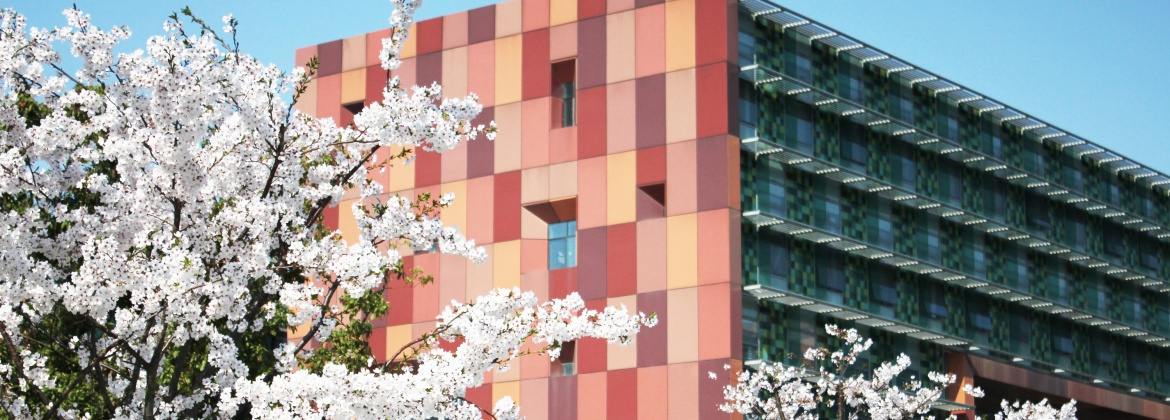
\includegraphics[height=\paperheight,width=\paperwidth,keepaspectratio=FALSE]{bgxp.jpg}};} % bdbg-1.jpeg

\titlegraphic{
\includegraphics[width=1.7cm]{xjtluicon.jpg}} %stat-right.png
